\hypertarget{a-common-frame-and-a-finite-response}{%
\section{A common frame and a finite response}\label{a-common-frame-and-a-finite-response}}

Consider a nonrotating orthonormal spatial frame carried by an expanding fiducial normal observer. We use signature \((-+++ )\), proper radial positions \(r n\), \(n\cdot n=1\), and the fixed scales

\[
\begin{aligned}
c &= 299792.458\ {\rm km\,s^{-1}}, & R_* &= 100\ {\rm Mpc},\\
v_* &= 300\ {\rm km\,s^{-1}}, & \beta_* &= v_*/c,\\
h_* &= v_*/R_* = 3\ {\rm km\,s^{-1}\,Mpc^{-1}}.
\end{aligned}\tag{1}
\]

Our dimensionless radial datum is \(y=(c/v_*)\delta z\). All vector components and tensors below refer to this same frame. The source bulk and observer velocities are \(v_*b\) and \(v_*\ell\). A positive observer velocity along the observer-to-source direction reduces the first-order radial redshift, giving the relative-motion term \(n\cdot(b-\ell)\). A scalar rate coefficient \(h_*m\) and a trace-free symmetric rate \(h_*S\) complete the local affine part of the response. These are coefficients of a local first-order design; the reference frame and scales do not supply a finite-redshift propagation law or an absolute background expansion measurement.

Choose the Frobenius-orthonormal STF basis

\[
\begin{aligned}
F_1&={\operatorname{diag}(1,-1,0)\over\sqrt2},&
F_2&={\operatorname{diag}(1,1,-2)\over\sqrt6},\\
F_3&={e_xe_y^T+e_ye_x^T\over\sqrt2},&
F_4&={e_xe_z^T+e_ze_x^T\over\sqrt2},&
F_5&={e_ye_z^T+e_ze_y^T\over\sqrt2}.
\end{aligned}                                                        \tag{2}
\]

Thus \(S=\sum_{a=1}^5s_aF_a\) and \(\|S\|_F^2=\sum_a s_a^2\). We retain all five signed coordinates and the full matrix, rather than its norm alone.

Let \(\tau\in[0,1]\) parametrize a stipulated two-mode matter-tilt history,

\[
\beta_G(\tau)=\beta_*[g_0+(2\tau-1)g_1].                 \tag{3}
\]

The coefficients \(g_0,g_1\) are dimensionless vectors in the transported common frame. For a normalized window \(W\), prescribe the dimensionless sensitivity

\[
\rho n\cdot\int_0^1 W(\tau){\beta_G(\tau)\over\beta_*}\,d\tau,
\qquad \rho={r\over R_*}.                               \tag{4}
\]

Equation (4) defines this experiment. It does not derive a universal relation between tilt, acceleration and a redshift-rate dipole. A physical application must provide that relation and its window independently. The illustrative coefficient box \([-1,1]^{18}\) ensures \(\sup_\tau\|\beta_G(\tau)\|\le2\sqrt3\beta_*<1\); the box serves only to locate the finite examples and is not a probability distribution or a cosmological admissible region.

Order the parameters as

\[
\theta=(\ell_x,\ell_y,\ell_z,b_x,b_y,b_z,m,
g_{0x},g_{0y},g_{0z},s_1,\ldots,s_5,g_{1x},g_{1y},g_{1z})^T.
                                                               \tag{5}
\]

For the baseline window \(W_0=1\), the integral of \(2\tau-1\) vanishes. With one free scalar calibration \(\alpha\), the thirteen baseline means are

\[
y_i=\alpha+n_i\cdot(b-\ell)
       +\rho_i[m+n_i\cdot g_0+n_i^TSn_i].                 \tag{6}
\]

The first nine directions, all at \(\rho=1\), are

\[
e_x,-e_x,e_y,-e_y,e_z,-e_z,
(3/5,4/5,0),(3/5,0,4/5),(0,3/5,4/5).                    \tag{7}
\]

Append \(e_x,-e_x,e_y,e_z\) at \(\rho=q>0\). The nominal design uses \(q=2\). Define \(E_3\) to have rows \(n_i^T\), define \(Q_5\) to have rows \((n_i^TF_an_i)_{a=1}^5\), and set \(R=\operatorname{diag}(\rho_i)\). The baseline design and nuisance column are

\[
J_0=[-E_3,\ E_3,\ R\mathbf1,\ RE_3,\ RQ_5,\ 0_{13\times3}],
\qquad N_0=\mathbf1_{13}.                                \tag{8}
\]

Here \(R\mathbf1\) is a vector of dimensionless radii; it is distinct from the physical length \(R_*\).

\hypertarget{one-nuisance-quotient-and-two-additional-responses}{%
\section{One nuisance quotient and two additional responses}\label{one-nuisance-quotient-and-two-additional-responses}}

Two independently calibrated three-component responses are proposed:

\[
z_L=\ell+e_L,\qquad
z_G=\int_0^1 2\tau\,{\beta_G(\tau)\over\beta_*}\,d\tau+e_G
     =g_0+{g_1\over3}+e_G.                              \tag{9}
\]

The first supplies an observer-velocity anchor. The second uses the normalized window \(W_1=2\tau\), whose overlap with \(2\tau-1\) is \(1/3\). Their declared gains express both in dimensionless \(y\)-equivalent units. This is a pair of hypothetical measurement functionals, rather than a claimed delivered survey channel. Their calibration is independent in the algebraic sense that neither carries the free \(\alpha\) of (6). No stochastic independence is assumed.

The augmented rows are

\[
J_L=[I_3,0,0,0,0,0],\qquad
J_G=[0,0,0,I_3,0,I_3/3],\qquad
J=\begin{pmatrix}J_0\\J_L\\J_G\end{pmatrix},\qquad
N=\begin{pmatrix}\mathbf1_{13}\\0_3\\0_3\end{pmatrix}.       \tag{10}
\]

Block widths in (10) follow (5). Removing an addition deletes its three rows from both \(J\) and \(N\). For every design, the scalar nuisance is removed once, using the complete retained data vector and the same construction for all parameter columns. For a positive row-precision matrix \(W\), define

\[
P=I-{(WN)(WN)^T\over\|WN\|^2},\qquad
A_{\rm phys}=PWJ,\qquad \bar y=PWy.                     \tag{11}
\]

For the full design we take

\[
W=\operatorname{diag}(I_{13},\sigma_L^{-1}I_3,
                                    \sigma_G^{-1}I_3),    \tag{12}
\]

with nominal \(\sigma_L=\sigma_G=1\). The subdesigns retain the applicable diagonal blocks. These positive scales define a deterministic comparison metric. A physical joint sampling covariance and a statistical law are not supplied. In particular, the singular-value plots below do not carry confidence levels.

The kernel characterization

\[
PWJ\theta=0\quad\Longleftrightarrow\quad J\theta\in\operatorname{col}N
                                                               \tag{13}
\]

holds because \(W\) is invertible and \(P\) projects away exactly \(WN\). Thus finite positive precision weights alter conditioning but not structural identifiability. Allowing unknown offsets for the added responses would enlarge \(N\) and require a new analysis.

\hypertarget{exact-ranks-and-identified-combinations}{%
\section{Exact ranks and identified combinations}\label{exact-ranks-and-identified-combinations}}

\textbf{Proposition 1 (two-radius separation).} For (7), the nine-dimensional spherical polynomial space consisting of a monopole, a dipole and an STF quadrupole is unisolvent. With the four repeated directions in (7) placed at any distinct positive radius \(q\ne1\), the matrix

\[
X=[E_4,RE_9],\qquad E_4=[\mathbf1,E_3],\quad
E_9=[\mathbf1,E_3,Q_5]                                  \tag{14}
\]

has rank thirteen.

\emph{Proof.} Let \(f(n)=a+d\cdot n+n^TTn\), \(T\) STF, vanish on the first nine directions. The opposite axis pairs first give \(d=0\), then \(a+T_{ii}=0\). Taking the trace gives \(a=0\) and all three diagonal entries vanish. At the three remaining directions the nonzero cross terms force \(T_{xy}=T_{xz}=T_{yz}=0\). Hence \(E_9\) is invertible. A degree-one polynomial vanishing at \(e_x,-e_x,e_y,e_z\) is likewise zero, so the repeated-direction \(E_4\) is invertible. A null vector of (14) represents polynomials \(p_1+\rho p_2\). At \(\rho=1\), unisolvence gives \(p_2=-p_1\) as polynomials. At the four repeated directions the equation becomes \((1-q)p_1=0\), forcing \(p_1=p_2=0\). This is the retained two-radius rank argument, expressed in the orthonormal tensor coordinates (2). \(\square\)

\textbf{Proposition 2 (baseline quotient).} At \(q\ne1\), the baseline response after (11) has rank twelve. Its exact six-dimensional kernel is

\[
k_{\rm split}(v)=(v,v,0,0,0,0),\qquad
k_{\rm hist}(w)=(0,0,0,0,0,w),\qquad v,w\in\mathbb R^3.    \tag{15}
\]

The identified signed combinations are

\[
b-\ell,\qquad m,\qquad g_0,\qquad(s_1,\ldots,s_5).       \tag{16}
\]

\emph{Proof.} By (13), a quotient-null vector satisfies \(J_0\theta=a\mathbf1\) for some \(a\). Proposition 1 applied to the coefficients \((-a,b-\ell,m,g_0,s)\) forces \(a=0\), \(b-\ell=0\), \(m=g_0=s=0\). No row contains \(g_1\). These are precisely (15), proving both completeness and the rank. \(\square\)

The ambiguity in (15) has two separate mechanisms. A shared change to source bulk and observer velocity leaves their relative radial velocity unchanged. A history proportional to \(2\tau-1\) has zero unweighted mean. Repeated angular or radial observations with the same response window cannot reveal that history coefficient.

\textbf{Proposition 3 (constructive augmentation).} At \(q\ne1\), either response in (9) gives quotient rank fifteen and a three-dimensional kernel. Their joint addition gives quotient rank eighteen and a unique eighteen-coordinate inverse on the quotient data image.

\emph{Proof.} The first addition acts on (15) as \(J_Lk_{\rm split}(v)=v\) and \(J_Lk_{\rm hist}(w)=0\). The second acts as \(J_Gk_{\rm split}(v)=0\) and \(J_Gk_{\rm hist}(w)=w/3\). Hence each addition removes exactly its corresponding three-dimensional kernel, and together they remove all six dimensions. Equation (13) extends the result to every positive finite precision weighting in (12). \(\square\)

This count separates information supplied by an endpoint anchor from information supplied by a new history moment. The same conclusion follows by reconstructing

\[
\ell=z_L,\qquad b=(b-\ell)+z_L,\qquad
g_1=3(z_G-g_0),                                         \tag{17}
\]

after solving for (16).

\textbf{Proposition 4 (equal-radius negative control).} At \(q=1\), the baseline quotient has rank eight. Either addition has rank eleven, and their joint addition has rank fourteen.

\emph{Proof.} At one radius, (6) depends only on the scalar \(\alpha+m\), the dipole \(b-\ell+g_0\), and the five STF coefficients. The nuisance quotient removes the scalar, leaving the independent dipole and quadrupole, hence rank eight. Each calibrated addition contributes three independent output coordinates. With both additions the remaining kernel is generated by

\[
\delta\theta_d=(0,-d,0,d,0,-3d),\qquad
\delta\theta_m=(0,0,t,0,0,0),\quad d\in\mathbb R^3, t\in\mathbb R.
                                                               \tag{18}
\]

The first leaves every raw mean, including both additions, unchanged. The second is absorbed by \(\delta\alpha=-t\). Conversely, a joint quotient-null vector obeys \(\ell=0\), \(g_1=-3g_0\), \(b=-g_0\) and \(s=0\), with \(m\) free. Thus the kernel has exactly four dimensions. \(\square\)

Equation (18) exhibits why independent endpoint and history anchors do not replace radial leverage. Distinct radii separate an angular intercept from a depth-proportional dipole and monopole.

\hypertarget{explicit-finite-witnesses}{%
\section{Explicit finite witnesses}\label{explicit-finite-witnesses}}

Starting from \(\theta=0\), choose \(v=e_x/4\) and \(w=e_y/4\). The two states \(k_{\rm split}(v)\) and \(k_{\rm hist}(w)\) both remain in the illustrative box. Every baseline prediction is exactly zero for each state. The first changes \(z_L\) by \((1/4,0,0)\); the second changes \(z_G\) by \((0,1/12,0)\). Their sum changes both additions while leaving all thirteen baseline means unchanged. These signed nineteen-coordinate predicted arrays are retained in the numerical supplement.

The history witness corresponds to

\[
\beta_G(\tau)={\beta_*\over4}(2\tau-1)e_y.               \tag{19}
\]

Its time integral vanishes although the history is nonzero except at its midpoint. The zero baseline column is therefore a response null direction, not a statement that the physical history vanishes.

For an equal-radius joint witness in the same box, take \(d=e_x/4\) in (18): \(b=-e_x/4\), \(g_0=e_x/4\), \(g_1=-3e_x/4\), with all other coordinates zero. All nineteen raw means remain zero. A separate change \(m=1/4\), \(\alpha=-1/4\) supplies the monopole witness.

\hypertarget{fixed-normalization-and-spectral-comparison}{%
\section{Fixed normalization and spectral comparison}\label{fixed-normalization-and-spectral-comparison}}

Velocity and rate scales in (1) are specified before numerical normalization. Let \(J_*\) and \(P_*\) denote the full design at \(q=2\), \(\sigma_L=\sigma_G=1\). Define once

\[
d_j=\|P_*J_*e_j\|_2>0,\qquad
L=\operatorname{diag}(d_1^{-1},\ldots,d_{18}^{-1}),\qquad
\theta=Lz.                                             \tag{20}
\]

The normalized response is

\[
A=PWJL.                                                 \tag{21}
\]

Nominal augmented columns have unit norm. The same numerical matrix \(L\) is then frozen for every subdesign, radius and precision case. In particular, the baseline's three zero history columns remain zero; weaker channels are not restored to unit norm during a scan. The supplement records the complete \(d_j\), \(L\), unscaled and scaled spectra and all physical unit conversions.

With \(A=U\Sigma V^T\), the identified scaled coordinates are \(V_r^Tz=V_r^TL^{-1}\theta\), where \(V_r\) contains the right singular vectors for the nonzero spectrum. The corresponding projector is \(\Pi_{\rm id}=V_rV_r^T\), and the kernel projector is \(I-\Pi_{\rm id}\). The named physical combinations (16) span the same identified information but are not an orthonormal singular-vector basis. Singular-vector signs and bases within repeated singular subspaces have no physical significance.

The baseline is a \(13\times18\) matrix of rank twelve. A thin SVD returns thirteen singular values and therefore only one explicit zero. The parameter kernel still has six dimensions. The complete eighteen-dimensional right basis and kernel projector are required to retain the five additional null directions absent from that thin list. The plotted spectrum may pad the missing five entries with structural zeros provided the caption identifies the padding.

The finite comparison uses the following analytic targets:

\begin{longtable}[]{@{}lrrrr@{}}
\toprule\noalign{}
Design & Rows & Rank at \(q=2\) & Kernel dimension & Rank at \(q=1\) \\
\midrule\noalign{}
\endhead
\bottomrule\noalign{}
\endlastfoot
Baseline & 13 & 12 & 6 & 8 \\
Baseline plus endpoint & 16 & 15 & 3 & 11 \\
Baseline plus history & 16 & 15 & 3 & 11 \\
Both additions & 19 & 18 & 0 & 14 \\
\end{longtable}

\begin{longtable}[]{@{}
  >{\raggedright\arraybackslash}p{(\columnwidth - 10\tabcolsep) * \real{0.1364}}
  >{\raggedleft\arraybackslash}p{(\columnwidth - 10\tabcolsep) * \real{0.1818}}
  >{\raggedleft\arraybackslash}p{(\columnwidth - 10\tabcolsep) * \real{0.1818}}
  >{\raggedleft\arraybackslash}p{(\columnwidth - 10\tabcolsep) * \real{0.1818}}
  >{\raggedleft\arraybackslash}p{(\columnwidth - 10\tabcolsep) * \real{0.1818}}
  >{\raggedright\arraybackslash}p{(\columnwidth - 10\tabcolsep) * \real{0.1364}}@{}}
\toprule\noalign{}
\begin{minipage}[b]{\linewidth}\raggedright
Design
\end{minipage} & \begin{minipage}[b]{\linewidth}\raggedleft
Rank
\end{minipage} & \begin{minipage}[b]{\linewidth}\raggedleft
Kernel
\end{minipage} & \begin{minipage}[b]{\linewidth}\raggedleft
Positive smin
\end{minipage} & \begin{minipage}[b]{\linewidth}\raggedleft
Identified condition
\end{minipage} & \begin{minipage}[b]{\linewidth}\raggedright
Full-vector gain
\end{minipage} \\
\midrule\noalign{}
\endhead
\bottomrule\noalign{}
\endlastfoot
baseline & 12 & 6 & 0.10665269 & 16.950054 & unbounded \\
endpoint & 15 & 3 & 0.097638737 & 18.655425 & unbounded \\
history & 15 & 3 & 0.10180602 & 17.900956 & unbounded \\
both & 18 & 0 & 0.093938751 & 19.539575 & 10.6452 \\
\end{longtable}

\begin{figure}[ht]
\centering
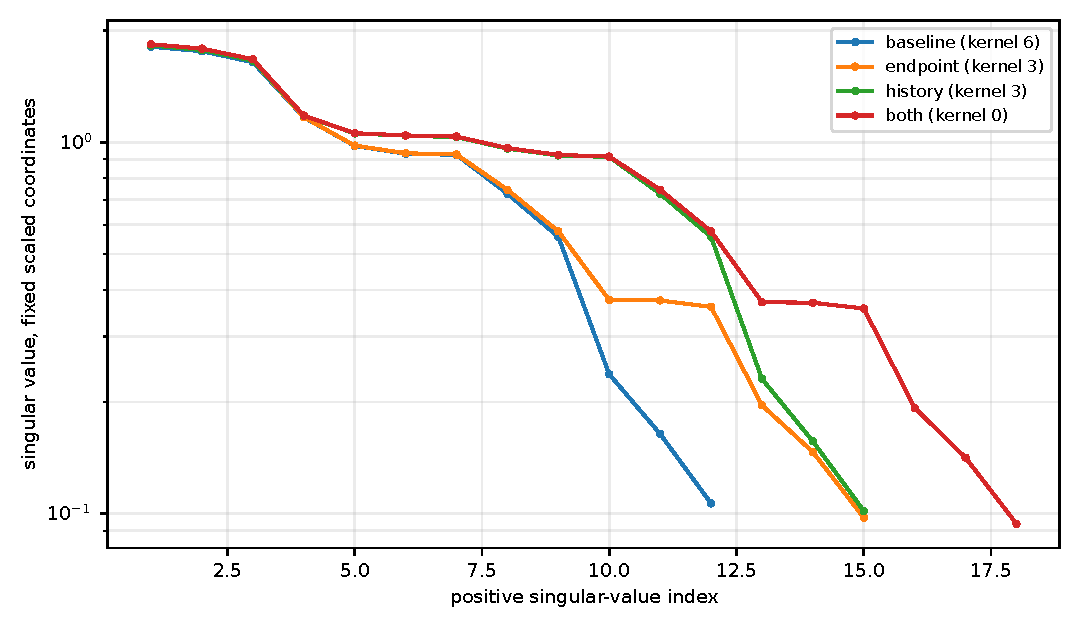
\includegraphics[width=0.95\linewidth]{figure1_spectra.pdf}
\caption{Singular spectra at q=2 with the fixed normalization (20). Legends state structural null dimensions. The row metric is stipulated, not measured covariance.}
\end{figure}

To show radial sensitivity, set \(q=1+\delta\) for

\[
\delta\in\{0,10^{-4},10^{-3},10^{-2},10^{-1},1,3\}.      \tag{22}
\]

At every positive separation, the analytic ranks are those of Proposition 3; as the separation approaches zero, four joint singular directions become weak and at equality join the exact kernel. Numerical threshold dependence near equality should be displayed alongside the structural rank. A finite threshold does not change the algebraic theorem. At equality the inverse gain for all eighteen coordinates is infinite, even though the fourteen identified directions retain finite gains.

For additional-channel precision, evaluate every pair

\[
(\sigma_L,\sigma_G)\in\{1/2,1,2,4\}^2                 \tag{23}
\]

at \(q=2\), preserving (20). These cases measure how the weakest recoverable combination responds to the relative precision of the two added channels.

\begin{figure}[ht]
\centering
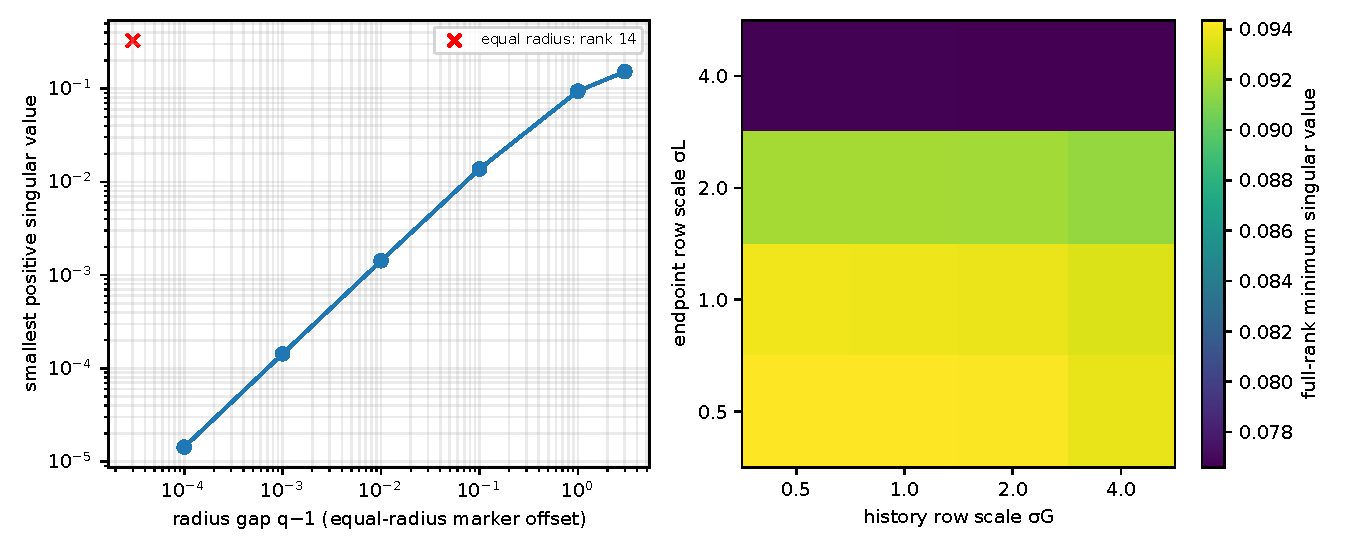
\includegraphics[width=0.95\linewidth]{figure2_leverage_precision.pdf}
\caption{Radial leverage and additional-channel precision in fixed scaled coordinates. The equal-radius marker is offset horizontally for log display; its full-vector inverse gain is unbounded.}
\end{figure}

\hypertarget{deterministic-error-sensitivity}{%
\section{Deterministic error sensitivity}\label{deterministic-error-sensitivity}}

Let the normalized projected data obey \(\bar y=Az+e\), with \(\|e\|_2\le\epsilon\). Suppose the operator used for inversion is \(\widetilde A=A+\Delta\), where \(\|\Delta\|_2\le\eta\). Both errors are measured after the prescribed quotient and normalization. Thus \(\Delta\) must include any error in that effective operator; nuisance-model changes cannot be treated as harmless coordinate changes. For a full-column-rank \(A\), Weyl's bound gives

\[
s_{\min}(\widetilde A)\ge s_{\min}(A)-\eta.             \tag{24}
\]

If \(s_{\min}(A)>\eta\), the least-squares inverse satisfies

\[
\|\widehat z-z\|_2
\le {\epsilon+\eta\|z\|_2\over s_{\min}(A)-\eta}.       \tag{25}
\]

\emph{Proof.} Full column rank of \(\widetilde A\) gives \(\widehat z-z=\widetilde A^+(e-\Delta z)\). Taking norms and using (24) proves (25). No distribution or independence assumption is used. \(\square\)

The physical coefficient error obeys \(\|\widehat\theta-\theta\|_2\le\|L\|_2\|\widehat z-z\|_2\), and any specified linear physical functional can use its own sharper factor \(\|CL\|_2\). The illustration \(\epsilon=10^{-3}\), \(\|z\|_2\le1\) is a separate error scenario, not the claim that the whole box \([-1,1]^{18}\) lies in the unit \(z\)-ball. For \(\eta/s_{\min}\in\{0,0.1,0.25,0.5,0.75,0.9,1,1.1\}\), the bound loses certification at one. Such cases are reported as \texttt{NOT\_CERTIFIED\_BY\_THIS\_BOUND}.

For a fixed rank-deficient operator, the minimum-norm estimate recovers the orthogonal identified projection with

\[
\|\widehat z-\Pi_{\rm id}z\|_2
\le{\epsilon\over s_{\min}^{+}(A)},                    \tag{26}
\]

where \(s_{\min}^{+}\) is the smallest nonzero singular value. This controls identified combinations only. An arbitrary kernel component leaves the data unchanged, so no uniform full-vector bound follows. Perturbations that change rank or the kernel require their own subspace control; (26) is the fixed-operator statement.

Equation (17) also gives direct, physically transparent bounds. If the errors on the estimated combinations obey \(\|\delta(b-\ell)\|\le e_D\), \(\|\delta z_L\|\le e_L\), \(\|\delta g_0\|\le e_0\), and \(\|\delta z_G\|\le e_G\), then

\[
\|\delta b\|\le e_D+e_L,\qquad
\|\delta g_1\|\le3(e_G+e_0).                           \tag{27}
\]

The history inverse incurs a factor of three because the new window overlaps the previously invisible temporal mode by only \(1/3\). This penalty survives the fact that the joint design is injective.

\begin{figure}[ht]
\centering
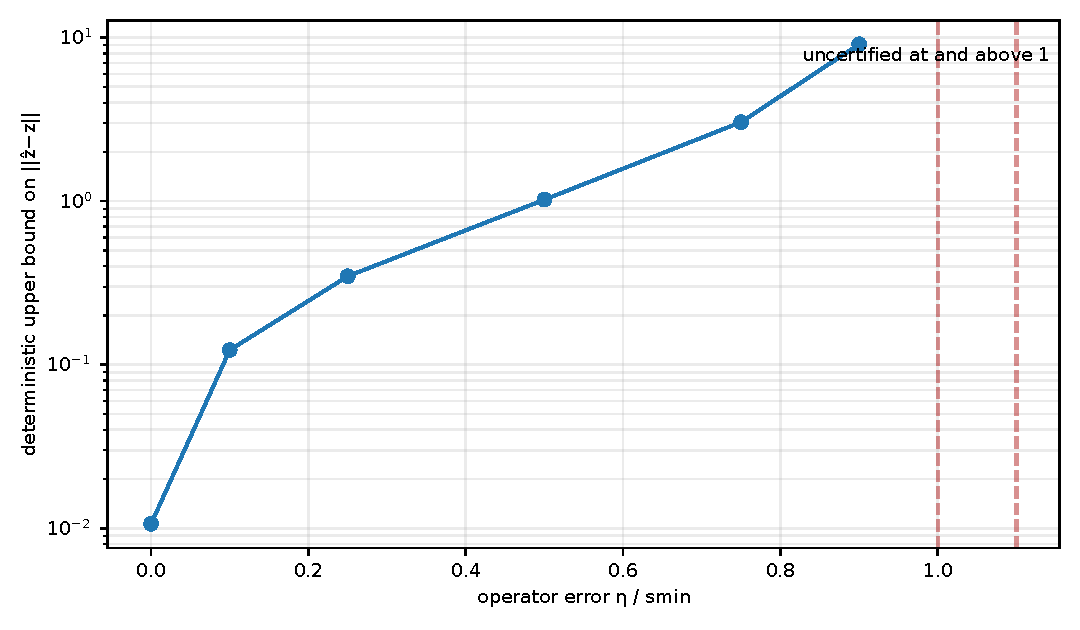
\includegraphics[width=0.95\linewidth]{figure3_error_bound.pdf}
\caption{Deterministic inverse bound (25) for epsilon=0.001 and ||z||<=1. At and above eta/smin=1 the bound is uncertified. No sampling law is supplied.}
\end{figure}

\hypertarget{physical-interpretation-and-the-next-measurement}{%
\section{Physical interpretation and the next measurement}\label{physical-interpretation-and-the-next-measurement}}

The design identifies what must change when a baseline response cannot separate physical mechanisms. The observer--bulk ambiguity requires a response to observer motion that is not a response to the same source bulk displacement. The history ambiguity requires a window with nonzero overlap with a temporal mode invisible to the existing window. These requirements are independent of the number of rows carrying the unchanged baseline response. Radial leverage performs a third job: separating angular intercepts from rate and mean-history coefficients.

For a physical implementation, the carrier remains the signed vectors \((\ell,b,g_0,g_1)\), the full STF tensor \(S\), scalar \(m\), response functions and their joint error set in one frame. The radial response contains no antisymmetric velocity-gradient measurement, because \(n^T\Omega n=0\). Matter vorticity therefore remains \texttt{NOT\_MEASURED}; a chosen hypersurface normal's irrotationality is a distinct statement. The scalar rate and fitted STF coefficients in this design do not alone provide a validated physical expansion/shear bridge.

No map from this finite carrier to a physical signed comparator \(x_C\), an anchored stress score \(Q\), an occupancy \(F\), an exceedance \(\Pi\), or a depth functional \(G_F\) has been specified. Each remains \texttt{NOT\_EVALUABLE\_WITH\_THIS\_RESPONSE}. Respectively, evaluation would require the full physical comparator components and frame, a sign/domain-clean anchor, a support measure and ceiling, a joint probability law, and compatible depth supports and joint dependence. These missing definitions are retained as undefined sectors rather than filled by zero.

The original V03 external-history validation remains a separate requirement. It must supply actual endpoint and history response kernels, calibration/nuisance coupling, common-frame transport and units, and a justified response error or covariance. The result here is the exact finite conditional design and its inverse sensitivity. It neither changes the original scientific acceptance nor supplies a native transfer or family-identification result.

\hypertarget{numerical-appendix-reproducible-comparison}{%
\appendix
\section{Numerical appendix: reproducible comparison}\label{numerical-appendix-reproducible-comparison}}

The companion consumer verifies the sealed retained inputs, constructs (2), (7)--(12), freezes (20), and emits all designs, full right singular bases, kernel/identified projectors, spectra and signed witnesses. The nominal rank counts must agree at relative cutoffs \(10^{-12},10^{-10},10^{-8}\). Frobenius-basis and null residuals must be at most \(10^{-12}\); reconstruction and deterministic bound checks use relative tolerance \(10^{-10}\) or absolute tolerance \(10^{-12}\) for unit-scale fixtures. Exact analytic rank remains authoritative near equal radii. The generated tables and figures report both numerical values and their design assumptions.

The source rank theorem is retained from \texttt{mathematical\_recovery.md}, ``Two radii separate angular nuisance and depth response'', corroborated in \texttt{independent\_review.md}, ``Rank-thirteen example and recovered physical scope'', and related to the oracle rank criterion in \texttt{NATIVE\_INFERENCE\_THEOREMS.md}, §6. The endpoint/history distinction and common nuisance quotient are developed in \texttt{theory\_synthesis\_20260913/REPORT.md}, §§13--13.1, and \texttt{theorem\_physical\_chapter.md}, the response quotient and anchor-coordinate paragraphs. Their precise source identities and the new finite construction are separated in the companion claim map.

\hypertarget{generated-numerical-appendix-tables}{%
\section{Generated numerical appendix tables}\label{generated-numerical-appendix-tables}}

\begin{longtable}[]{@{}llrr@{}}
\toprule\noalign{}
Parameter & Physical coefficient unit & d\_j & L\_jj \\
\midrule\noalign{}
\endhead
\bottomrule\noalign{}
\endlastfoot
ell\_x & v*=300 km/s & 2.368381466 & 0.4222292795 \\
ell\_y & v*=300 km/s & 2.134695078 & 0.4684509794 \\
ell\_z & v*=300 km/s & 2.181742423 & 0.4583492485 \\
b\_x & v*=300 km/s & 2.146911915 & 0.4657852952 \\
b\_y & v*=300 km/s & 1.885980667 & 0.5302281287 \\
b\_z & v*=300 km/s & 1.939071943 & 0.5157106231 \\
m & h*=3 km/s/Mpc & 1.664100589 & 0.6009252126 \\
g0\_x & beta*=300/299792.458 & 3.407232127 & 0.2934933584 \\
g0\_y & beta*=300/299792.458 & 2.666602563 & 0.3750090147 \\
g0\_z & beta*=300/299792.458 & 2.698717644 & 0.3705463601 \\
s\_1 & h*=3 km/s/Mpc & 2.8381359 & 0.3523439452 \\
s\_2 & h*=3 km/s/Mpc & 2.664247621 & 0.3753404872 \\
s\_3 & h*=3 km/s/Mpc & 0.6521915717 & 1.533291817 \\
s\_4 & h*=3 km/s/Mpc & 0.6521915717 & 1.533291817 \\
s\_5 & h*=3 km/s/Mpc & 0.6521915717 & 1.533291817 \\
g1\_x & beta*=300/299792.458 & 0.3333333333 & 3 \\
g1\_y & beta*=300/299792.458 & 0.3333333333 & 3 \\
g1\_z & beta*=300/299792.458 & 0.3333333333 & 3 \\
\end{longtable}

\hypertarget{complete-nominal-scaled-spectrum-baseline}{%
\subsection{Complete nominal scaled spectrum: baseline}\label{complete-nominal-scaled-spectrum-baseline}}

\begin{longtable}[]{@{}rr@{}}
\toprule\noalign{}
Index & Singular value \\
\midrule\noalign{}
\endhead
\bottomrule\noalign{}
\endlastfoot
1 & 1.80776894878 \\
2 & 1.75783553205 \\
3 & 1.64202991241 \\
4 & 1.16693241497 \\
5 & 0.977608148968 \\
6 & 0.93153934285 \\
7 & 0.925000426039 \\
8 & 0.72695402196 \\
9 & 0.556681575992 \\
10 & 0.237422793074 \\
11 & 0.164010989736 \\
12 & 0.106652693887 \\
13 & 2.28393497472e-16 \\
14 & structural zero (right completion) \\
15 & structural zero (right completion) \\
16 & structural zero (right completion) \\
17 & structural zero (right completion) \\
18 & structural zero (right completion) \\
\end{longtable}

\hypertarget{complete-nominal-scaled-spectrum-endpoint}{%
\subsection{Complete nominal scaled spectrum: endpoint}\label{complete-nominal-scaled-spectrum-endpoint}}

\begin{longtable}[]{@{}rr@{}}
\toprule\noalign{}
Index & Singular value \\
\midrule\noalign{}
\endhead
\bottomrule\noalign{}
\endlastfoot
1 & 1.8214921072 \\
2 & 1.77388823641 \\
3 & 1.6579048791 \\
4 & 1.16814162944 \\
5 & 0.979221208186 \\
6 & 0.933867897306 \\
7 & 0.92679745181 \\
8 & 0.745208194267 \\
9 & 0.57589372613 \\
10 & 0.375920041292 \\
11 & 0.375052692147 \\
12 & 0.360409875835 \\
13 & 0.195900842657 \\
14 & 0.146618339872 \\
15 & 0.097638736537 \\
16 & 0 \\
17 & structural zero (right completion) \\
18 & structural zero (right completion) \\
\end{longtable}

\hypertarget{complete-nominal-scaled-spectrum-history}{%
\subsection{Complete nominal scaled spectrum: history}\label{complete-nominal-scaled-spectrum-history}}

\begin{longtable}[]{@{}rr@{}}
\toprule\noalign{}
Index & Singular value \\
\midrule\noalign{}
\endhead
\bottomrule\noalign{}
\endlastfoot
1 & 1.8224251976 \\
2 & 1.77075892464 \\
3 & 1.6569969902 \\
4 & 1.17889465675 \\
5 & 1.05629533648 \\
6 & 1.04195741167 \\
7 & 1.03219924361 \\
8 & 0.961460443345 \\
9 & 0.921463617644 \\
10 & 0.91312580769 \\
11 & 0.726700364284 \\
12 & 0.55634543484 \\
13 & 0.230754137695 \\
14 & 0.1566639275 \\
15 & 0.101806023814 \\
16 & 1.84960232996e-16 \\
17 & structural zero (right completion) \\
18 & structural zero (right completion) \\
\end{longtable}

\hypertarget{complete-nominal-scaled-spectrum-both}{%
\subsection{Complete nominal scaled spectrum: both}\label{complete-nominal-scaled-spectrum-both}}

\begin{longtable}[]{@{}rr@{}}
\toprule\noalign{}
Index & Singular value \\
\midrule\noalign{}
\endhead
\bottomrule\noalign{}
\endlastfoot
1 & 1.83552330269 \\
2 & 1.78615342167 \\
3 & 1.6720014412 \\
4 & 1.17933809547 \\
5 & 1.05743023017 \\
6 & 1.04292085192 \\
7 & 1.03553442499 \\
8 & 0.964471288015 \\
9 & 0.924256501433 \\
10 & 0.914865452434 \\
11 & 0.745162919861 \\
12 & 0.57555461857 \\
13 & 0.371204892219 \\
14 & 0.36975411719 \\
15 & 0.356918568169 \\
16 & 0.192824411934 \\
17 & 0.141550104788 \\
18 & 0.0939387506842 \\
\end{longtable}

All arrays, complete right bases and source-linked checks are in the companion JSON artifacts. This numerical appendix is generated from the frozen design and does not add observed channels.
